\begin{frame}
\begin{tabular}{cc}
\psset{xunit=0.3cm,yunit=0.3cm}
\begin{pspicture*}(-7,-10)(7,10)%
\pstVerb{20 dict begin}%
\pstVerb{/pi 3.141592654 def}%
\psaxes[labels=none, ticks=x, Dx=1.570796327] {<->}(0,0)(-7,-10)(7,10)%
\tiny%
\rput[lt](5.5,0){$x$}%
\rput[lb](0.2,9){$y$}%
%\rput[t](1,-0.1){1}
\psline[linecolor=gray](1,-0.1)(1,0.1) % x unit mark
\rput[lb](1.570796327,0.1){$\frac{\pi}2$}%
\psline[linecolor=gray](1.570796327,-0.1)(1.570796327,0.1) % pi/2 unit mark
\psline[linecolor=gray](-0.1,1)(0.1,1) % y unit mark
\pstVerb{/xShift 0 def /flip 1 def}%
\only<handout:0|3->{\pstVerb{/xShift pi 6 div def}}%
\only<handout:0|4->{\pstVerb{/xShift pi 3 div def}}%
\only<handout:2|5->{\pstVerb{/xShift pi 2 div def}}%
\only<handout:2|6->{\pstVerb{/flip -1 def}}%
\psplot[linecolor=red]{pi -0.5 mul xShift sub 0.1 add}{pi 0.5 mul xShift sub -0.1 add}{x xShift add 180 mul pi div tan flip mul} 
\psplot[linecolor=red]{pi -1.5 mul xShift sub 0.1 add}{pi -0.5 mul xShift sub -0.1 add}{x xShift add 180 mul pi div tan flip mul} 
\psplot[linecolor=red]{pi 0.5 mul xShift sub 0.1 add}{pi 1.5 mul xShift sub -0.1 add}{x xShift add 180 mul pi div tan flip mul} 
\only<handout:2|3->{
\psplot[linecolor=gray!50]{-1.57 pi 0 mul add}{1.57 pi 0 mul add}{x 180 mul pi div tan} 
\psplot[linecolor=gray!50]{-1.57 pi -1 mul add}{1.57 pi -1 mul add}{x 180 mul pi div tan} 
\psplot[linecolor=gray!50]{-1.57 pi 1 mul add}{1.57 pi 1 mul add}{x 180 mul pi div tan} 
}


\psline[linestyle=dotted](-4.71238898,-10)(-4.71238898,10)
\psline[linestyle=dotted](-1.570796327,-10)(-1.570796327,10)
\psline[linestyle=dotted](1.570796327,-10)(1.570796327,10)
\psline[linestyle=dotted](4.71238898,-10)(4.71238898,10)
\pstVerb{end}
\end{pspicture*}
%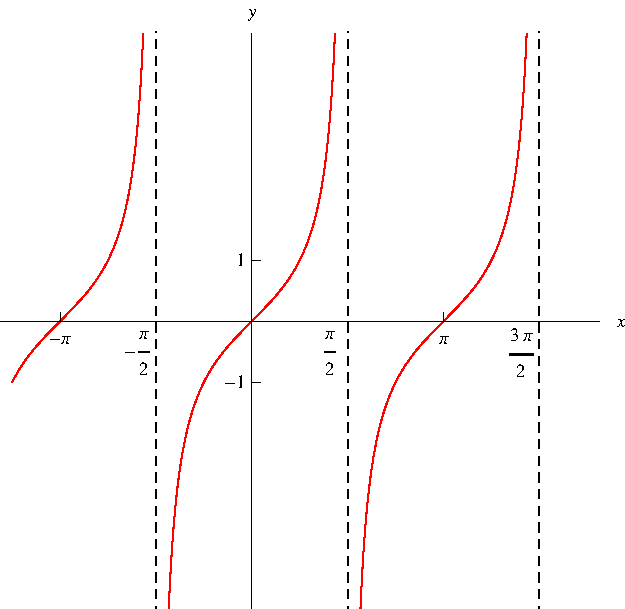
\includegraphics[width=5.5cm]{trigonometry/pictures/app-d-tan.pdf}%

&%
\psset{xunit=0.3cm,yunit=0.3cm}
\begin{pspicture*}(-7,-10)(8,10)
\tiny
\pstVerb{20 dict begin}
\pstVerb{/pi 3.141592654 def}
\psaxes[labels=none, ticks=x, Dx=1.570796327] {<->}(0,0)(-7,-10)(7,10)
\rput[lt](7,0){$x$}
\rput[lb](0.2,9){$y$}
%\rput[t](1,-0.1){1}
\psline[linecolor=gray](1,-0.1)(1,0.1) % x unit mark
\rput[rb](3.13,0.1){$\pi$}
\psline[linecolor=gray](1.570796327,-0.1)(1.570796327,0.1) % pi/2 unit mark
%\rput[br](0,1){1}
\psline[linecolor=gray](-0.1,1)(0.1,1) % y unit mark
\psplot[linecolor=red]{0.01}{3.14}{1 180 x mul  3.1415 div tan div} 
\psplot[linecolor=red]{3.15}{6.28}{1 180 x mul  3.1415 div tan div} 
\psplot[linecolor=red]{-3.14}{-0.01}{1 180 x mul  3.1415 div tan div} 
\psplot[linecolor=red]{-6.28}{-3.15}{1 180 x mul  3.1415 div tan div} 
%\psplot[linecolor=red]{-4.71}{-1.58}{ 180 x mul  3.1415 div cot} 
%\psplot[linecolor=red]{1.58}{4.71}{ 180 x mul  3.1415 div cot} 
\psline[linestyle=dotted](-6.283185307,-10)(-6.283185307,10)
\psline[linestyle=dotted](-3.141592654,-10)(-3.141592654,10)
\psline[linestyle=dotted](3.141592654,-10)(3.141592654,10)
\psline[linestyle=dotted](6.283185307,-10)(6.283185307,10)
\pstVerb{end}
\end{pspicture*}
%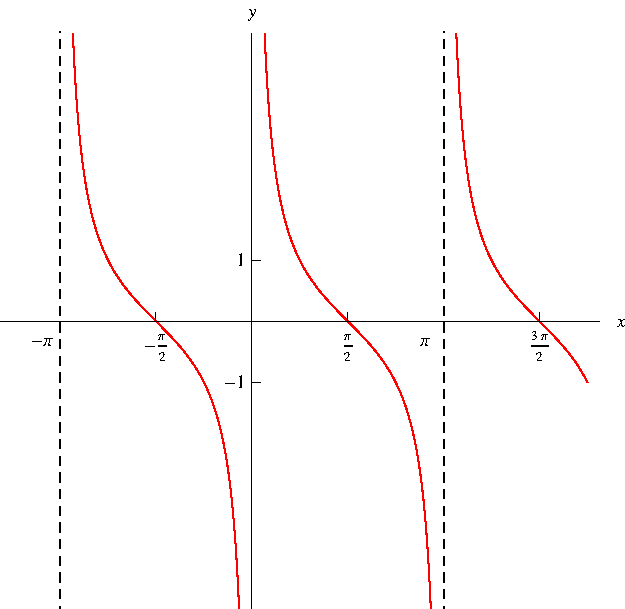
\includegraphics[width=5.5cm]{trigonometry/pictures/app-d-cot.pdf}%
\\%
$y = \tan x$ & $y = \cot x$\\
\end{tabular}

\uncover<2->{If we move the graph of $\tan x$ by $\frac{\pi}{2}$ units to the left (or right) and reflect across the $x$ axis}\uncover<6->{, we get the graph of $\cot x$.} \uncover<7->{This follows from $\tan \left(x\pm \frac{\pi}{2}\right) =-\cot x$.}\uncover<handout:2|0>{}
\end{frame}
